\subsection*{ISO-Kriterium Aufgabenangemessenheit}
\begin{figure}[H]
    \centering
    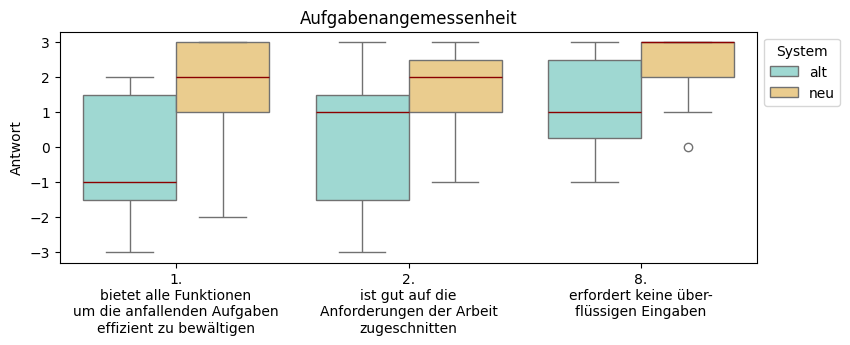
\includegraphics[width=1\linewidth]{Diagramme/pruemper_aa.png}
    \caption{Auswertung der Fragen bzgl. Gestaltungskriterium Aufgabenangemessenheit nach ISO 9241-110 (Ausschnitt aus \autoref{fig:pruemper_all})}
    \label{fig:pruemper_Aufgabenangemessenheit}
\end{figure}

\noindent
t-Test von Fragen 1 \& 8 sind signifikant (<0.5)\\
wenn bei 2 die beiden Ausreißer weggenommen werden, die andersrum bewertet haben, dann wird der Unterschied auch signifikant (s. \autoref{fig:hist_prümper_all})\\
Boxplot: \autoref{fig:pruemper_Aufgabenangemessenheit}